\section{Conclusion}
	\begin{itemize}
	\item In this chapter, we have presented a background of current approaches that deal with the integration of heterogeneous models and languages in both a structural and a behavioral way. 
	
	\item We presented several approaches that enables the composition of structures. Some approaches specify the composition at language level but apply between models thus automating the composition of structural models. Other enables the composition of languages structure in order to obtain a new syntax.  
	
	\item We have noted that the MDE community provides some extensive support for the structural composition of models and languages.
	
	\item Afterwards, we have presented the state of art approaches that deal with the integration of behaviors. We have identified two approaches that relay on different mechanisms to obtain the emerging system behavior: Composition and Coordination. 
	
	\item We have determined that compositional approaches only provides support for the composition of homogeneous behavioral models. Differently, coordination approaches also give support for the coordination of heterogeneous behavioral models. 
	
	\item Then, we have presented the work done by Coordination Languages and ADLs in order to coordinate the behavior of heterogeneous models. Afterwards, we have shown how coordination pattern approaches have leveraged on the know-how of system designer to automate the coordination of models. 
	
	\item However, we have noted that the knowledge about system integration is currently either implicitly held by the system designer or encoded within a framework. 
	
	\item To capture explicitly this knowledge and thus leverage integrator know-how, we propose a dedicated language to capture coordination patterns between languages, thus reifying the coordination specification at the language level.    

	\item In the next chapter, we use the concepts from this chapter to define a multi-view framework to model systems
	\end{itemize}


         	\begin{figure}
         		\begin{center}
         			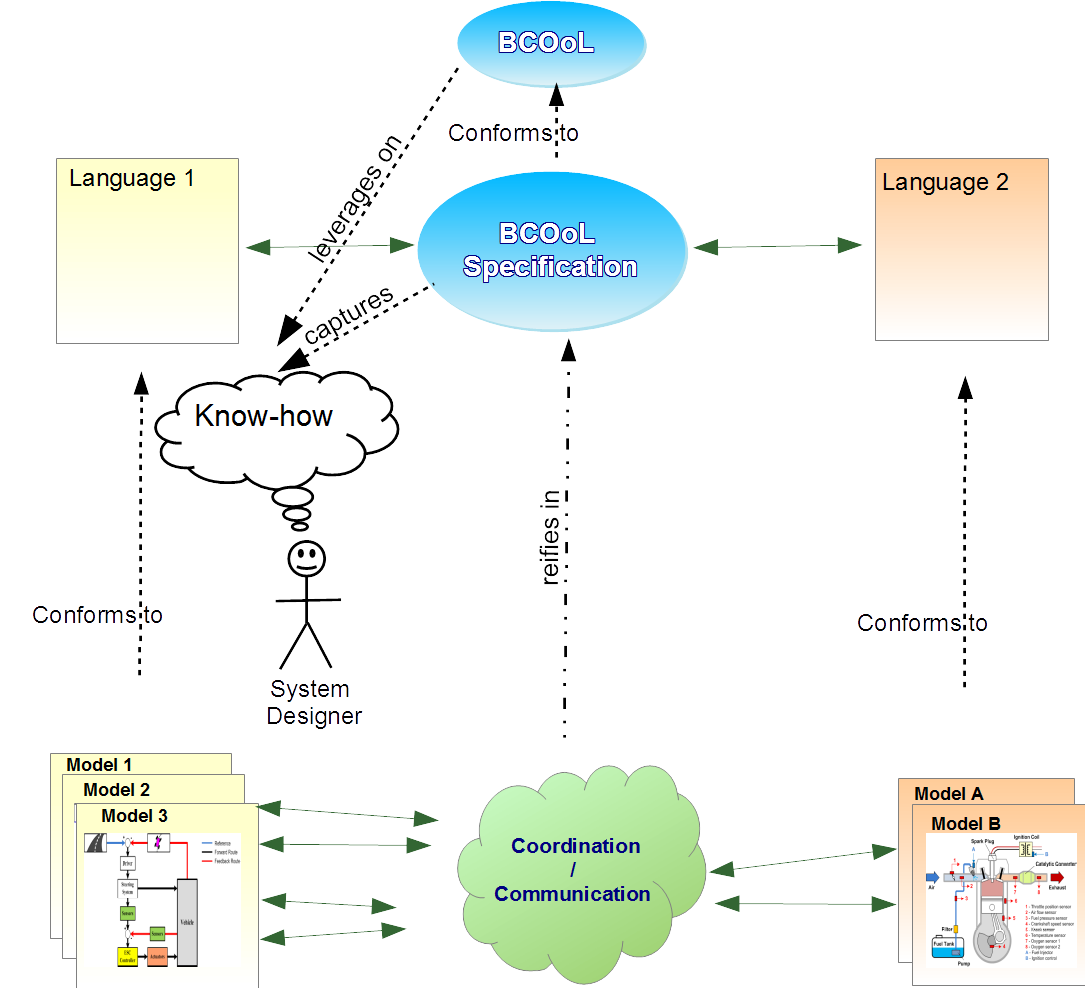
\includegraphics[width=0.7\textwidth]{background/figs/bcoolapp.png}
         			\caption{Overview of Our Approach}
         			\label{fig:bcoolapp}
         		\end{center}
         	\end{figure}	


\begin{landscape}% Landscape page

\begin{table}[]
	\centering
	\caption{Overview of Behavioral Approaches}
	\label{my-label}
	\resizebox{\textwidth}{!}{%
		\begin{tabular}{cllcccccc
				>{\columncolor[HTML]{9AFF99}}l }
			\multicolumn{3}{c}{} Approaches & Semantic Anchoring & \cite{compostatechartsbib} & Esper & Rapide & Ptolemy & Di Natale et. al & BCOoL \\
			\multicolumn{3}{c}{Syntactic Composition} &  &  &  &  &  &  &  \\
			\multicolumn{3}{c}{Behavioral Composition} & X (Homogeneous) & \begin{tabular}[c]{@{}c@{}}X \\ (Homogeneous)\end{tabular} &  &  &  &  &  \\
			\multicolumn{3}{c}{\cellcolor[HTML]{FFFE65}Behavioral Coordination} &  &  & X (N Models) & X (N Models) & \cellcolor[HTML]{FFFE65}X(predefined Languages) & \cellcolor[HTML]{FFFE65}X (2 Languages) & X (N Languages) \\
			\multicolumn{3}{c}{\cellcolor[HTML]{FFCC67}Language used to express the coordination between Models} & Assml & Statechart & \cellcolor[HTML]{FFCC67}Formal Language & \cellcolor[HTML]{FFCC67}Formal Language & JAVA in a framework & C++ in a framework & Formal Language
		\end{tabular}
	}
\end{table}
\end{landscape}
